\documentclass[12pt]{beamer}

% Tema da apresentação
\usetheme{Madrid}
\usecolortheme{default}

% Pacotes necessários
\usepackage[utf8]{inputenc}
\usepackage[portuguese]{babel}
\usepackage{amsmath}
\usepackage{amsfonts}
\usepackage{amssymb}
\usepackage{graphicx}
\usepackage{url}
\usepackage{hyperref}

% Configurações para resolver problemas de layout
\setbeamertemplate{navigation symbols}{}
\setbeamertemplate{footline}[frame number]
\tolerance=1000
\emergencystretch=3em

% Informações da apresentação
\title[Plano Inclinado de Galileu]{Determinação da Aceleração da Gravidade através do Plano Inclinado de Galileu Galilei}
\subtitle{Física Experimental I}
\author{Grupo 6 - ECO2025.2 \\ Johnnathan Victor Gonçalves Sabbá \\ Nelson Dias Ponciano Scarin}
\institute{Instituto Federal Catarinense}
\date{\today}

% Logo da instituição
\titlegraphic{
\includegraphics[width=2cm]{pictures/brasao.png}}

\begin{document}

% Slide de título
\begin{frame}
    \titlepage
\end{frame}

% Sumário
\begin{frame}{Sumário}
    \tableofcontents
\end{frame}

% Seção 1: Introdução Histórica
\section{Introdução Histórica}

\begin{frame}{Galileu Galilei (1564-1642)}
    \begin{columns}
        \begin{column}{0.6\textwidth}
            \begin{itemize}
                \item Pai da física experimental moderna
                \item Desafiou a visão aristotélica
                \item Desenvolveu o método científico
                \item Introduziu a matemática na física
            \end{itemize}
        \end{column}
        \begin{column}{0.4\textwidth}
            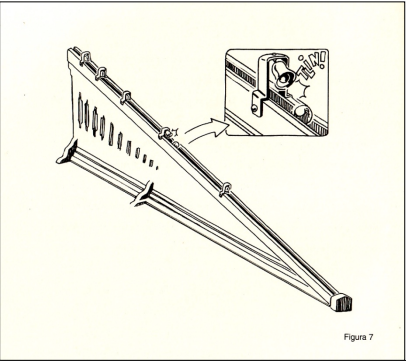
\includegraphics[width=\textwidth]{pictures/GalileuPlano.png}
        \end{column}
    \end{columns}
\end{frame}

\begin{frame}{O Problema de Galileu}
    \begin{block}{Desafio Tecnológico}
        Como medir o tempo de queda livre com a tecnologia do século XVII?
    \end{block}

    % \pause

    \begin{block}{Solução Genial}
        \begin{itemize}
            \item Usar um plano inclinado para "dilatar" o tempo
            \item Reduzir a aceleração: $a = g \cdot \sin(\theta)$
            \item Permitir medições mais precisas
        \end{itemize}
    \end{block}
\end{frame}

% Seção 2: Materiais e Métodos
\section{Materiais e Métodos}

\begin{frame}{Montagem Experimental}
    \begin{center}
        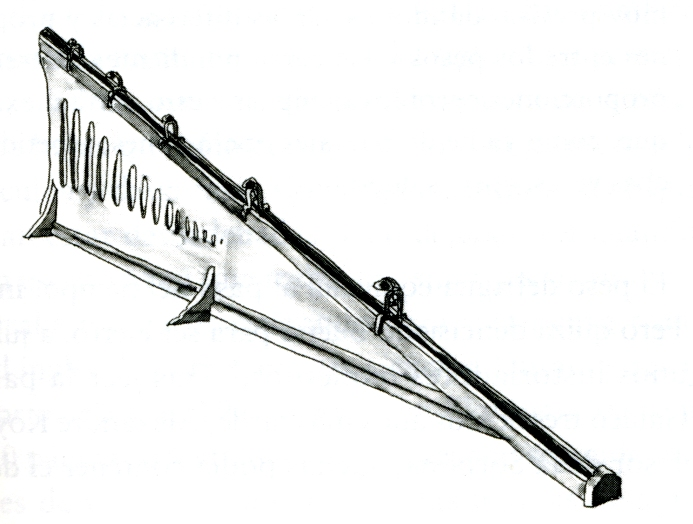
\includegraphics[width=0.8\textwidth]{pictures/planoInclinado.png}
    \end{center}
\end{frame}

\begin{frame}{Materiais Utilizados}
    \begin{itemize}
        \item \textbf{Rampa:} fio de nylon (1 m)
        \item \textbf{Objetos em queda:} Porcas e braçadeiras metálicas
        \item \textbf{Cronômetro:} Digital (precisão: 0,01 s)
        \item \textbf{Trena:} Métrica (precisão: 1 mm)
        \item \textbf{Transferidor:} Para ângulos
              % \item \textbf{Suporte:} Ajuste de altura
    \end{itemize}
\end{frame}

\begin{frame}{Procedimento Experimental}
    \begin{enumerate}
        \item Montagem do plano inclinado em diferentes ângulos (30°, 60°)
        \item Calibração do sistema
        \item Medições de tempo para diferentes distâncias
        \item Repetição de cada medida (10 vezes)
        \item Registro e análise dos dados
    \end{enumerate}

    \begin{block}{Equação Fundamental}
        $$s = \frac{1}{2}at^2$$
    \end{block}
\end{frame}

% Seção 3: Física do Experimento
\section{Conceitos Físicos}

\begin{frame}{Decomposição de Forças}
    \begin{columns}
        \begin{column}{0.5\textwidth}
            \begin{align}
                F_{\parallel} & = mg \sin(\theta) \\
                F_{\perp}     & = mg \cos(\theta) \\
                a             & = g \sin(\theta)
            \end{align}
        \end{column}
        \begin{column}{0.5\textwidth}
            \begin{center}
                % Diagrama de forças seria inserido aqui
                \textit{Diagrama de forças no plano inclinado}
            \end{center}
        \end{column}
    \end{columns}
\end{frame}

\begin{frame}{Cinemática do Movimento}
    \begin{block}{Movimento Uniformemente Variado}
        \begin{align}
            v   & = v_0 + at = at \quad (v_0 = 0)             \\
            s   & = v_0 t + \frac{1}{2}at^2 = \frac{1}{2}at^2 \\
            v^2 & = v_0^2 + 2as = 2as
        \end{align}
    \end{block}

    \begin{block}{Determinação de g}
        $$g = \frac{a}{\sin(\theta)} = \frac{2s}{t^2 \sin(\theta)}$$
    \end{block}
\end{frame}

% \begin{frame}{Conservação de Energia}
%     \begin{block}{Transformação Energética}
%         \begin{align}
%             E_{p,inicial} & = mgh                                       \\
%             E_{c,final}   & = \frac{1}{2}mv^2                           \\
%             mgh           & = \frac{1}{2}mv^2 \quad \text{(sem atrito)}
%         \end{align}
%     \end{block}

%     \pause

%     \begin{alertblock}{Para Rolamento (sem deslizamento)}
%         $$E_c = \frac{1}{2}mv^2 + \frac{1}{2}I\omega^2$$
%         onde $I = \frac{2}{5}mr^2$ para esfera sólida
%     \end{alertblock}
% \end{frame}

% Seção 4: Resultados
\section{Resultados}

\begin{frame}{Dados Experimentais - Plano Inclinado 30°}
    \small
    \begin{columns}
        \begin{column}{0.5\textwidth}
            \begin{table}
                \centering
                \begin{tabular}{|c|c|}
                    \hline
                    \textbf{Tentativa} & \textbf{Tempo (s)} \\
                    \hline
                    1                  & 0,68               \\
                    2                  & 0,71               \\
                    3                  & 0,69               \\
                    4                  & 0,72               \\
                    5                  & 0,70               \\
                    \hline
                \end{tabular}
            \end{table}
        \end{column}
        \begin{column}{0.5\textwidth}
            \begin{table}
                \centering
                \begin{tabular}{|c|c|}
                    \hline
                    \textbf{Tentativa} & \textbf{Tempo (s)} \\
                    \hline
                    6                  & 0,69               \\
                    7                  & 0,73               \\
                    8                  & 0,71               \\
                    9                  & 0,70               \\
                    10                 & 0,68               \\
                    \hline
                \end{tabular}
            \end{table}
        \end{column}
    \end{columns}

    \vspace{0.3cm}
    \begin{block}{Resultados}
        \centering
        \textbf{Tempo médio:} $\bar{t} = 0,701$ s \\
        \textbf{Distância:} $s = 1,0$ m \\
        \textbf{Ângulo:} $\theta = 30^\circ$
    \end{block}
\end{frame}

\begin{frame}{Dados Experimentais - Plano Inclinado 60°}
    \small
    \begin{columns}
        \begin{column}{0.5\textwidth}
            \begin{table}
                \centering
                \begin{tabular}{|c|c|}
                    \hline
                    \textbf{Tentativa} & \textbf{Tempo (s)} \\
                    \hline
                    1                  & 0,41               \\
                    2                  & 0,40               \\
                    3                  & 0,42               \\
                    4                  & 0,39               \\
                    5                  & 0,43               \\
                    \hline
                \end{tabular}
            \end{table}
        \end{column}
        \begin{column}{0.5\textwidth}
            \begin{table}
                \centering
                \begin{tabular}{|c|c|}
                    \hline
                    \textbf{Tentativa} & \textbf{Tempo (s)} \\
                    \hline
                    6                  & 0,41               \\
                    7                  & 0,40               \\
                    8                  & 0,42               \\
                    9                  & 0,41               \\
                    10                 & 0,40               \\
                    \hline
                \end{tabular}
            \end{table}
        \end{column}
    \end{columns}

    \vspace{0.3cm}
    \begin{block}{Resultados}
        \centering
        \textbf{Tempo médio:} $\bar{t} = 0,410$ s \\
        \textbf{Distância:} $s = 0,58$ m \\
        \textbf{Ângulo:} $\theta = 60^\circ$
    \end{block}
\end{frame}

\begin{frame}{Cálculo da Aceleração da Gravidade}
    \begin{block}{Para 30°}
        \small
        \begin{align}
            a_{30} & = \frac{2s}{t^2} = \frac{2 \times 1,0}{(0,701)^2} = 4,07 \text{ m/s}^2  \\
            g_{30} & = \frac{a_{30}}{\sin(30^\circ)} = \frac{4,07}{0,5} = 8,14 \text{ m/s}^2
        \end{align}
    \end{block}

    \begin{block}{Para 60°}
        \small
        \begin{align}
            a_{60} & = \frac{2s}{t^2} = \frac{2 \times 0,58}{(0,410)^2} = 6,90 \text{ m/s}^2   \\
            g_{60} & = \frac{a_{60}}{\sin(60^\circ)} = \frac{6,90}{0,866} = 7,97 \text{ m/s}^2
        \end{align}
    \end{block}

\end{frame}

\begin{frame}{Análise dos Resultados}
    \begin{itemize}
        \item \textbf{Valor teórico:} $g = 9,81 \text{ m/s}^2$
        \item \textbf{Resultado para 30°:} $g = 8,14 \text{ m/s}^2$ (erro: 17,0\%)
        \item \textbf{Resultado para 60°:} $g = 7,97 \text{ m/s}^2$ (erro: 18,8\%)
        \item \textbf{Valor médio:} $g = 8,06 \text{ m/s}^2$ (erro: 17,9\%)
    \end{itemize}

    \begin{block}{Velocidades Finais}
        \begin{itemize}
            \item \textbf{Para 30°:} $v_f = 2,85 \text{ m/s}$ (usando $v = at$)
            \item \textbf{Para 60°:} $v_f = 2,83 \text{ m/s}$ (usando $v = at$)
        \end{itemize}
    \end{block}

    \begin{block}{Fontes de Erro}
        \begin{itemize}
            \item Tempo de reação humano no cronômetro
            \item Inclinação da haste de sustentação devido a tensão do sistema
            \item Atrito no sistema de sustentação
            \item Imprecisões na medição do ângulo
            \item Oscilações do objeto durante a queda
        \end{itemize}
    \end{block}
\end{frame}

% Seção 5: Aplicações
\section{Aplicações Práticas}

\begin{frame}{Aplicações no Cotidiano}
    \begin{block}{Engenharia Civil}
        \begin{itemize}
            \item Projeto de rampas de acesso
            \item Análise de taludes e encostas
            \item Sistemas de drenagem urbana
        \end{itemize}
    \end{block}

    \begin{block}{Indústria}
        \begin{itemize}
            \item Esteiras transportadoras
            \item Sistemas de escoamento (silos)
            \item Controle de qualidade automotivo
        \end{itemize}
    \end{block}
\end{frame}

\begin{frame}{Tecnologia Moderna}
    \begin{block}{Setor Automobilístico}
        \begin{itemize}
            \item Sistemas de freio ABS
            \item Controle de estabilidade (ESP)
            \item Testes de capotamento
        \end{itemize}
    \end{block}

    \begin{block}{Tecnologia Espacial}
        \begin{itemize}
            \item Trajetórias de lançamento
            \item Reentrada atmosférica
            \item Rovers em terrenos inclinados
        \end{itemize}
    \end{block}
\end{frame}

% Seção 6: Conclusões
\section{Conclusões}

\begin{frame}{Lições Aprendidas}
    \begin{block}{Metodologia Científica}
        \begin{itemize}
            \item Importância da experimentação controlada
            \item Técnicas de minimização de erros
            \item Análise estatística de dados
        \end{itemize}
    \end{block}

    \begin{block}{Pensamento Físico}
        \begin{itemize}
            \item Modelagem de sistemas complexos
            \item Decomposição de problemas
            \item Validação experimental de teorias
        \end{itemize}
    \end{block}
\end{frame}

\begin{frame}{Relevância Histórica e Atual}
    \begin{itemize}
        \item \textbf{Marco histórico:} Nascimento da física experimental
        \item \textbf{Método científico:} Base da ciência moderna
        \item \textbf{Aplicações tecnológicas:} Princípios presentes em diversas áreas
        \item \textbf{Valor didático:} Experimento simples, conceitos profundos
    \end{itemize}

    \begin{center}
        \textit{"E contudo ela se move"} - Galileu Galilei
    \end{center}
\end{frame}

% Slide de agradecimentos
\begin{frame}
    \begin{center}
        \Huge Obrigado!

        \vspace{1cm}

        \Large Perguntas?

        \vspace{1cm}

        \normalsize
        Grupo 6B - ECO2025.2 \\
        Física Experimental I \\
        Instituto Federal Catarinense
    \end{center}
\end{frame}

% Referências
\begin{frame}[allowframebreaks]{Referências}
    \tiny
    \begin{thebibliography}{99}
        \bibitem{galilei1988}
        GALILEI, G. \textbf{Discursos e demonstrações matemáticas sobre duas novas ciências}. São Paulo: Nova Stella, 1988.

        \bibitem{halliday2016}
        HALLIDAY, D.; RESNICK, R.; WALKER, J. \textbf{Fundamentos de Física}: Mecânica. 10. ed. Rio de Janeiro: LTC, 2016. v. 1.

        \bibitem{nussenzveig2013}
        NUSSENZVEIG, H. M. \textbf{Curso de Física Básica}: Mecânica. 5. ed. São Paulo: Blucher, 2013. v. 1.

        \bibitem{tipler2009}
        TIPLER, P. A.; MOSCA, G. \textbf{Física para cientistas e engenheiros}: Mecânica, oscilações e ondas, termodinâmica. 6. ed. Rio de Janeiro: LTC, 2009. v. 1.

        \bibitem{young2016}
        YOUNG, H. D.; FREEDMAN, R. A. \textbf{Física I}: Mecânica. 14. ed. São Paulo: Pearson, 2016.
    \end{thebibliography}
\end{frame}

\end{document}
